\usetikzlibrary{arrows.meta}
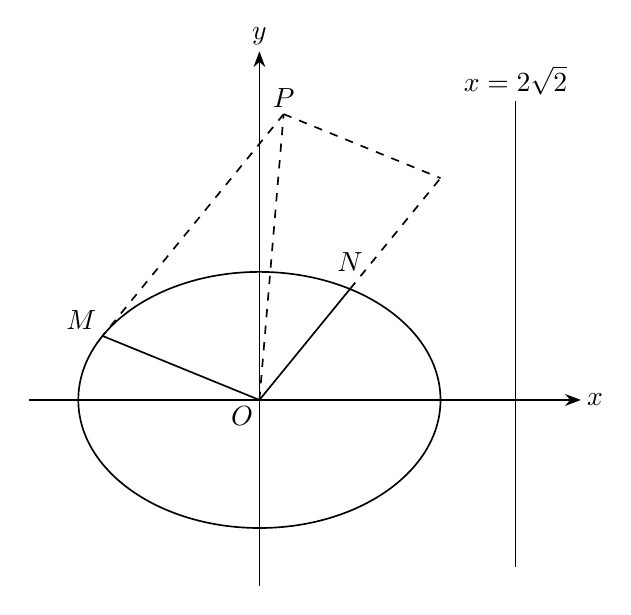
\begin{tikzpicture}[x=1.15cm,y=1.15cm,line width=.6pt,font=\normalsize,>=Stealth]
% axes
\draw[->] (-2.55,0)--(3.55,0) node[right,inner sep=0pt,xshift=2pt] {$x$};
\draw[->] (0,-2.05)--(0,3.85) node[above,inner sep=0pt,yshift=2pt] {$y$};
% ellipse x^2/4+y^2/2=1
\draw (0,0) ellipse[x radius=2,y radius=1.414214];
% directrix x=2sqrt2
\draw (2.828427,-1.85)--(2.828427,3.30);
\coordinate (O) at (0,0);
\coordinate (M) at (-1.732051,0.707107);
\coordinate (N) at (1,1.224745);
\coordinate (P) at (0.267949,3.156597);
\coordinate (N2) at (2,2.449490);
% solid radii OM and ON
\draw (O)--(M);
\draw (O)--(N);
% dashed parallelogram O-M-P-(2N) and diagonal OP
\draw[dashed] (O)--(P);
\draw[dashed] (P)--(M);
\draw[dashed] (P)--(N2);
\draw[dashed] (N)--(N2);
% labels kept clear of every drawn stroke
\node[below left,inner sep=0pt,xshift=-2pt,yshift=-2pt] at (O) {$O$};
\node[above left,inner sep=0pt,xshift=-2pt,yshift=2pt] at (M) {$M$};
\node[above,inner sep=0pt,yshift=6pt] at (N) {$N$};
\node[above,inner sep=0pt,yshift=2pt] at (P) {$P$};
\node[above,inner sep=0pt,yshift=2pt] at (2.828427,3.30) {$x=2\sqrt{2}$};
\end{tikzpicture}
